\subsubsection{monolith::client::events::ChecklistCompleteEmitter}

\label{monolith::client::events::ChecklistCompleteEmitter}
\begin{figure}[H]
	\centering
	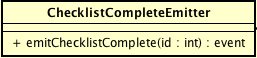
\includegraphics[scale=0.5]{Sezioni/SottosezioniST/img/ChecklistCompleteEmitter.png}
	\caption{monolith::client::events::ChecklistCompleteEmitter}
\end{figure}

\begin{itemize}
\item \textbf{Descrizione:} Classe che contiene l'emettitore di eventi da lanciare quando una checklist viene completata. Estende Event-Emitter (es6-event-emitter).
\item \textbf{Utilizzo:} La classe viene utilizzata ogniqualvolta una checklist viene completata, lanciando l'evento corrispondente.
\item \textbf{Attributi:}
\item \textbf{Metodi:}
\begin{itemize}
\item \textit{public emitChecklistComplete(id:string):void}\\
Questo metodo emette l'evento relativo al completamento di una lista.
			\\ \textbf{Parametri}: \begin{itemize}
			\item \textit{id:string}\\
			L'identificativo della lista che è stata completata
			\end{itemize} 
\end{itemize}
\end{itemize}

\subsubsection{monolith::client::events::ChecklistUpdateEmitter}

\label{monolith::client::events::ChecklistUpdateEmitter}
\begin{figure}[H]
	\centering
	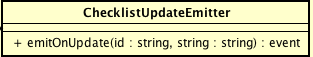
\includegraphics[scale=0.5]{Sezioni/SottosezioniST/img/ChecklistUpdateEmitter.png}
	\caption{monolith::client::events::ChecklistUpdateEmitter}
\end{figure}

\begin{itemize}
\item \textbf{Descrizione:} Classe che contiene l'emettitore di eventi da lanciare quando gli elementi di una checklist vengono cliccati. Estende Event-Emitter (es6-event-emitter).
\item \textbf{Utilizzo:} La classe viene utilizzata ogniqualvolta un elemento di una checklist viene cliccato, lanciando l'evento corrispondente.
\item \textbf{Attributi:}
\item \textbf{Metodi:}
\begin{itemize}
\item \textit{public emitOnUpdate(id:string,string:string):void}\\
Questo metodo emette l'evento relativo al click di un elemento di una lista.
			\\ \textbf{Parametri}: \begin{itemize}
			\item \textit{id:string}\\
			L'identificativo della lista della quale è stato cliccato un elemento.
			\item \textit{string:string}\\
			Stringa che contiene l'informazione relativa al tipo di click effettuato, se normale o prolungato.
			\end{itemize} 
\end{itemize}
\end{itemize}

\subsubsection{monolith::client::events::ClickButtonEventEmitter}

\label{monolith::client::events::ClickButtonEventEmitter}
\begin{figure}[H]
	\centering
	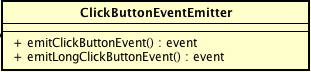
\includegraphics[scale=0.5]{Sezioni/SottosezioniST/img/ClickButtonEventEmitter.png}
	\caption{monolith::client::events::ClickButtonEventEmitter}
\end{figure}

\begin{itemize}
\item \textbf{Descrizione:} Classe che contiene l'emettitore di eventi da lanciare quando un bottone viene cliccato. Estende Event-Emitter (es6-event-emitter).
\item \textbf{Utilizzo:} La classe viene utilizzata ogniqualvolta un bottone viene cliccato.
\item \textbf{Attributi:}
\item \textbf{Metodi:}
\begin{itemize}
\item \textit{public emitClickButtonEvent():void}\\
Questo metodo emette l'evento relativo al click di un bottone.
\item \textit{public emitLongClickButtonEvent():void}\\
Questo metodo emette l'evento relativo al click prolungato di un bottone.
\end{itemize}
\end{itemize}